
Integration and system testing is the last phase of the project. In the previous section, it was presented the implementations that were made during the project and some unit tests that were performed for each module. Now, all modules of the system will be integrated and tested together in order to validate the all process.

\subsection{Generation and validation of the final system}

As mentioned in the beginning of this report, the DBT was modeled by four groups, each one with a different responsibilities. Therefore, a main component of the DBT was assigned to each group and the general ones were created by all. All the interfaces and general elaboration files were outlined as well by all groups. \\

Having the elaboration files created for each component of the model, the first steps was to check the generation of the final system. For that, the \textbf{SpecificElaborations} folder was filled with all elaboration associated with the source files annotated and the batch files \texttt{BuildSystem.bat} and \texttt{runElaborator.bat} were executed. The default values of the properties were maintained. A folder called \textbf{FinalFiles} were generated with all final sources, as illustrated in figure \ref{fig:final_files}.


\begin{figure}[H]
\centerline{
\includegraphics[scale=0.65]{images/finalfiles}
}
\caption{Generated (final) files.}
\label{fig:final_files}
\end{figure}

All sources were opened and it was verified that the annotations were replaced. To validate the source files modification, those were used to build a project in the IAR workbench and compiled to check if there was any error.

\begin{figure}[H]
\centerline{
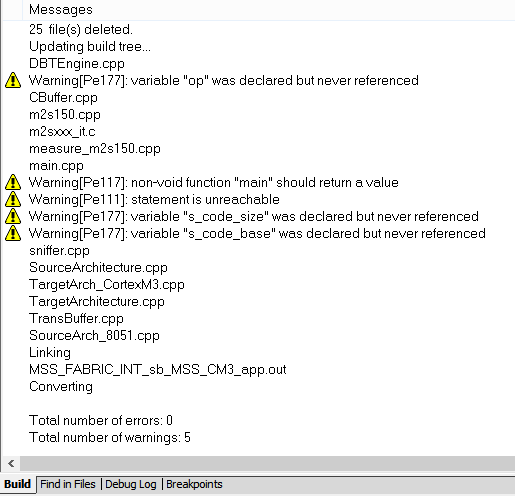
\includegraphics[scale=0.5]{images/compilar}
}
\caption{Compilation of the generated files.}
\label{fig:final_files2}
\end{figure}

It can be seen in figures \ref{fig:annotation_test1}, \ref{fig:annotation_test2}, \ref{fig:annotation_test3} that the replacement of the annotations was  a success. The examples demonstrates replacements in the \texttt{SourceArch\_8051.cpp} (figure \ref{fig:annotation_test1}), \texttt{TransBuffer.cpp} (figure \ref{fig:annotation_test2}) and in the \texttt{DBTEngine.cpp} (figure \ref{fig:annotation_test3}) files.

\begin{figure}[H]
\centerline{
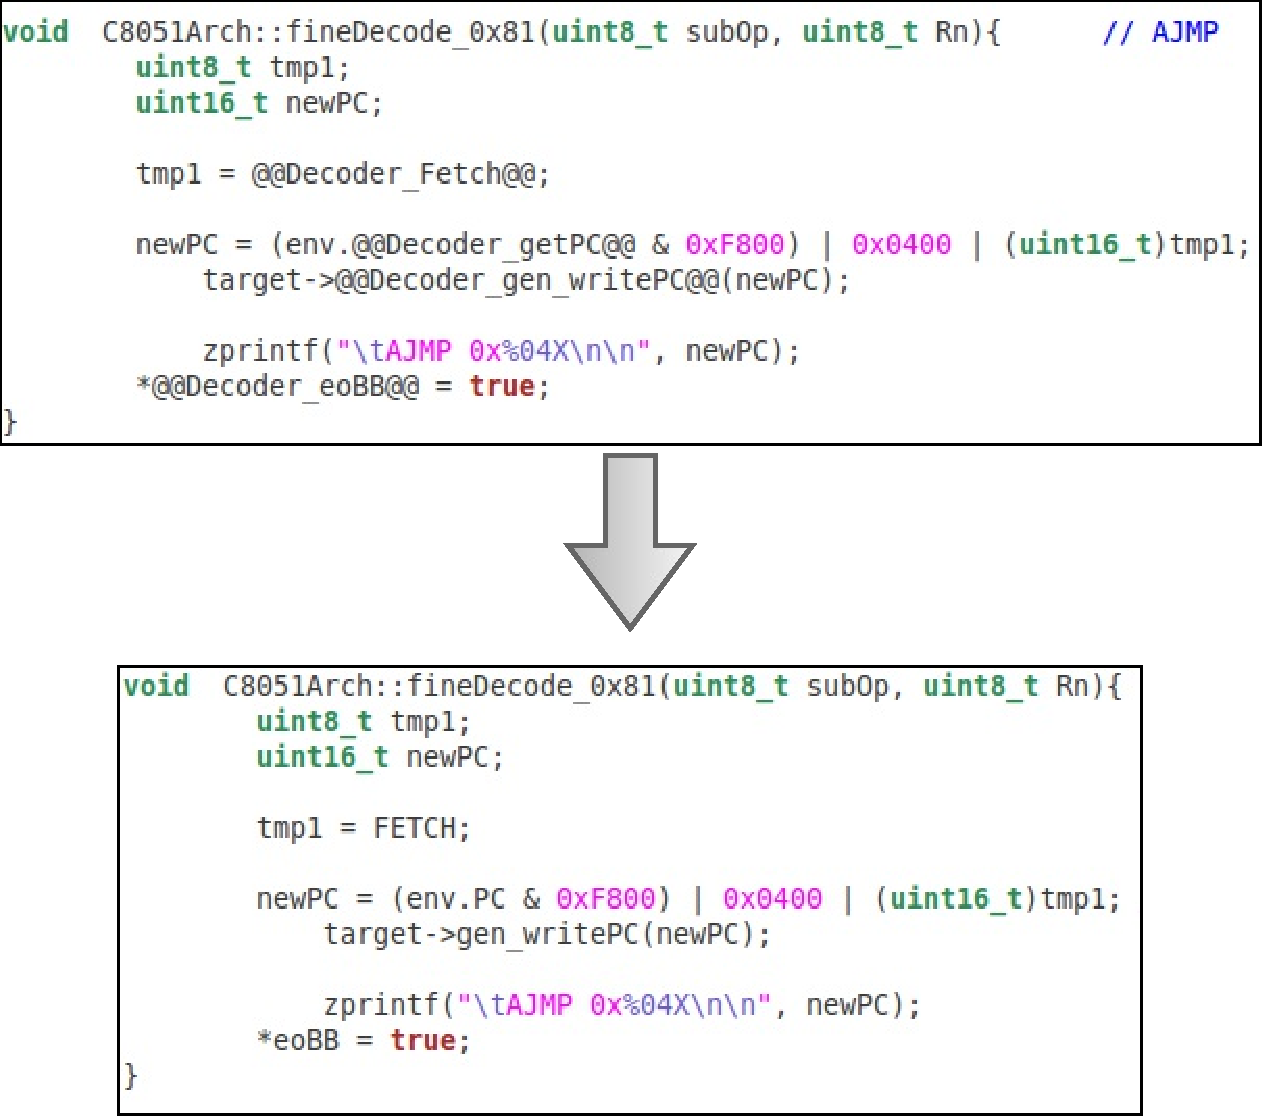
\includegraphics[scale=0.4]{images/annotation_test1}
}
\caption{Annotations replaced in the \texttt{SourceArch\_8051.cpp}.}
\label{fig:annotation_test1}
\end{figure}

\begin{figure}[H]
\centerline{
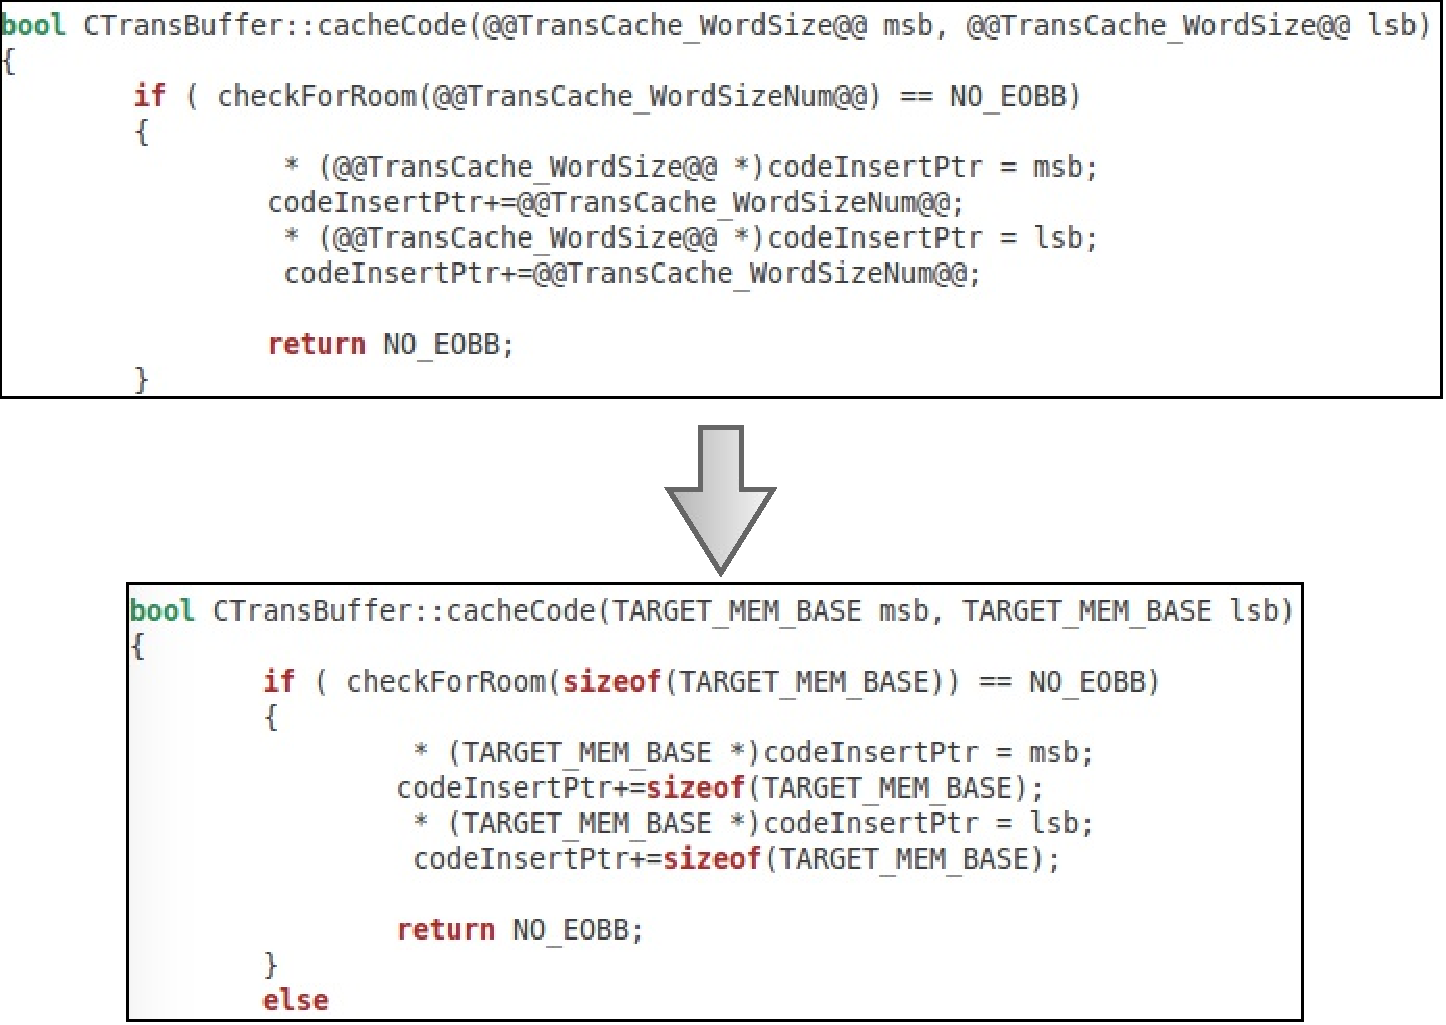
\includegraphics[scale=0.5]{images/annotation_test2}
}
\caption{Annotations replaced in the \texttt{TransBuffer.cpp}.}
\label{fig:annotation_test2}
\end{figure}

\begin{figure}[H]
\centerline{
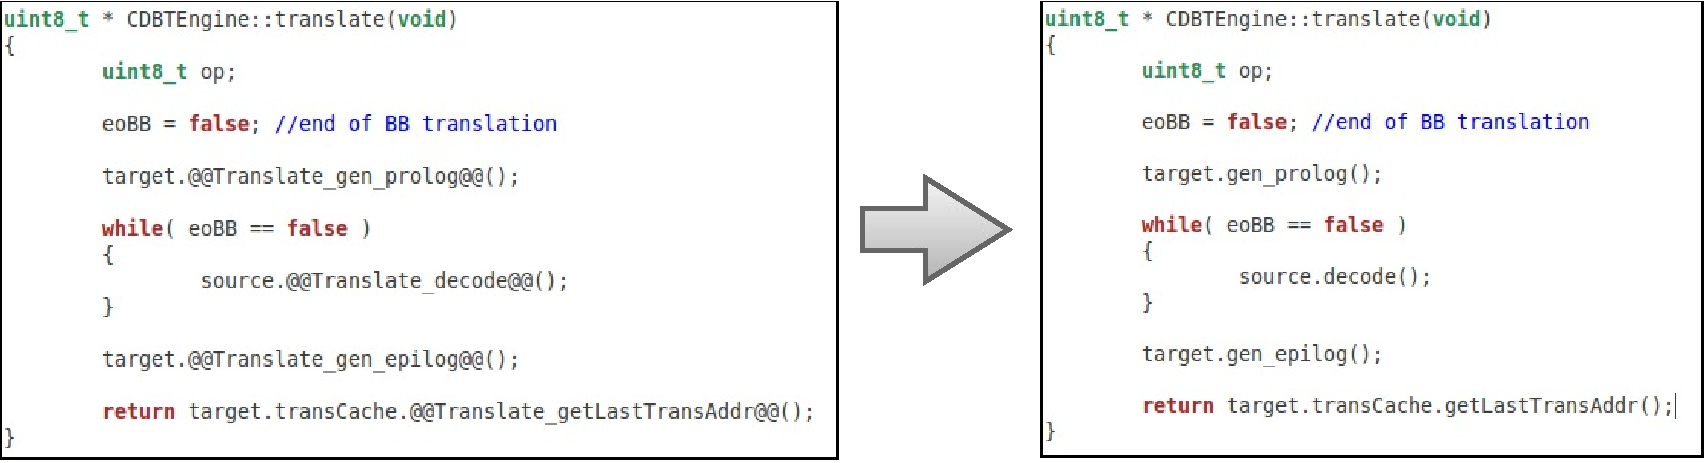
\includegraphics[scale=0.5]{images/annotation_test3}
}
\caption{Annotations replaced in the \texttt{DBTEngine.cpp} .}
\label{fig:annotation_test3}
\end{figure}


\subsection{Global Tests}

In order to prove the proper functioning of the system, tests under different configurations were made. Some tests can prove in which of those configurations the DBT works better and others only evidence the correct operation. 
Next, it will be shown experiments in each component of the DBT system and the results that allow the validation of the project.

\subsubsection{Decoder Tests}
The three elaboration files of the Decoder component (switch case, jump table and generic) were used in the generation of three final systems. A simple test was carried to evaluate the performance of the behaviors. A simulated source code to be translated was created as it can be seen in figure \ref{fig:SourceCodeDecoderTest}.

\begin{figure}[H]
\centerline{
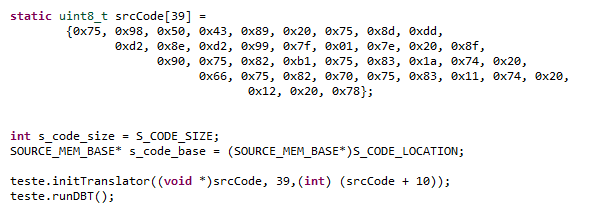
\includegraphics[scale=0.65]{images/sourceCode.png}
}
\caption{Simulated source code.}
\label{fig:SourceCodeDecoderTest}
\end{figure}

After running the system to each decoder behavior, under the same conditions, it was possible to discover the faster decoder.

\begin{figure}[H]
\centerline{
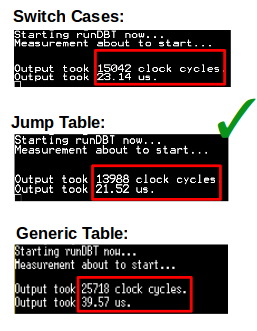
\includegraphics[scale=0.67]{images/DecoderBehaviorsResults}
}
\caption{Decoder Behaviors Measurements.}
\label{fig:DecoderBehaviorsMeasurements}
\end{figure}

As it can be seen in figure \ref{fig:DecoderBehaviorsMeasurements} the decoder based on a Jump Table presented a better result. The Generic Table decoder, due to all the overhead that carries, presented a considerable translate time.

\subsubsection{Code Tracing Tests}

Some properties were changed in the XML files of different components. The next test shows the system running varying two properties of the Generator and Decoder: \texttt{trgCodeTarcing} and \texttt{srcCodeTracing}. The result are shown in figure \ref{fig:finalteste}.

\begin{figure}[H]
\centerline{
\includegraphics[scale=0.5]{images/finalteste}
}
\caption{Tests disabling Source and Target code tracing.}
\label{fig:finalteste}
\end{figure}


The left image on the figure shows the log obtained when the system runs with the \texttt{trgCodeTrecing} set to false. This way, only the information about the translation is printed on the screen (only source instructions are presented). In the right image, the log obtained does not have code tracing for the source architecture (only translated instructions are presented). \\

The next test consists in changing the value of the property Measure in the DBT xml file. This will turn off all the logs when the DBT is running. That can be checked in figure \ref{fig:val4}.

\begin{figure}[H]
\centerline{
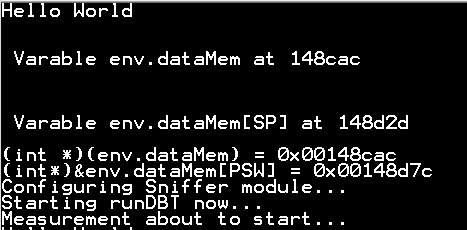
\includegraphics[scale=0.6]{images/val4}
}
\caption{Tests enabling measure property.}
\label{fig:val4}
\end{figure}

\subsubsection{Optimizations Tests}

\par The group developed a simple algorithm to reduce the overhead in the translated code and to prove that the model would be consistent enough when adding configuration points. This didn't affect the reference architecture of the dynamic binary translator and it was only needed to add on property to the \texttt{Generator} component to active/deactivate the optimizations.
\par When studying how the code was generated for the target architecture, that was detected the occurrence of irrelevant load instructions (Listing \ref{lst:ldst}). The situation is easily understandable in the next example that shows the translated code for the source instruction \texttt{INC DPTR}.
\begin{lstlisting}[language={[x86masm]Assembler},caption=Fragment of the generated code from DBT.,label=lst:ldst]
;R4 is the memory base and to it is added an offset

;Load of the contents of (R4,#82) to R5.	
LDRH R5,[R4,#82]
;Incremenent the value of R5.
ADDW R5, R5, #1
;Store the value of R5 in (R4 + #0x82) position
STRH R5, [R4 + #0x82]
;Load the value of (R4, #0x82) to R5
LDRB R5,[R4,#0x82]
\end{lstlisting}

\par The Load is not necessary in this situation because the value of R5 did not change between instructions. To save some cycles, it was introduced on simple algorithm to the load and store operations.
\par When a store instruction occurs, the value of the PC is stored into a auxiliar variable \texttt{auxPC\_Source}. The information about the register being used to store and the memory position are also stored into the variables \texttt{Optim\_DReg} and \texttt{auxR5} respectively (Listing \ref{lst:storeopt}). 

\begin{lstlisting}[language=C++,caption=Store function optimization code.,label=lst:storeopt]
#if OPTIMIZATION == true
auxPC_source = env->PC;
Optim_DReg = SReg;
auxR5 = imm; 
#endif
\end{lstlisting}
\par When a load instruction occurs, the register is compared with the value of \texttt{Optim\_DReg} and the immediate with the value stored in \texttt{auxR5}. Then, if the condition is true, it is verified if the actual PC is not more than three positions forward. This condition is necessary due to the variable size of the source architecture instructions' size. 
\par If this condition is true, then the value of \texttt{auxR5} is cleaned and the function ends here. There is no need to load from memory because the value of the register is valid (Listing \ref{lst:loadopt}). 

\begin{lstlisting}[language=C++,caption=Load function optimization code.,label=lst:loadopt]
#if OPTIMIZATION == true
if (DReg == Optim_DReg && auxR5 == imm){
if (auxPC_source == ((env->getPC)-1) || auxPC_source == ((env->PC)-2) || auxPC_source == ((env->PC)-3)){
auxR5 |= 0xffff;
return;
}
}
#endif 
\end{lstlisting}

\par With this simple algorithm, the number of cycles is reduced in more than 1.45\% when compared to the number of cycles executed when the optimizations are turned off. The group made various tests to the algorithm to conclude that it was the best approach. Table \ref{tab:opt} shows the different results.

\begin{table}[H]
	\centering
	\caption{Optimizations results.}
	\label{tab:opt}
	\begin{tabular}{l|lll}
		\hline
		\textbf{Description} & \begin{tabular}[c]{@{}l@{}}\textbf{Number} \\ \textbf{of cycles}\end{tabular} & \begin{tabular}[c]{@{}l@{}}\textbf{Exit} \\ \textbf{address}\end{tabular} & \begin{tabular}[c]{@{}l@{}}\textbf{Overhead} \\ \textbf{Reduction}\end{tabular} \\ \hline
		Without optimization & 11393410026 & 0x88f & 0\% \\
		\begin{tabular}[c]{@{}l@{}}With the first optimization \\ approach\end{tabular} & 11381943769 & 0x88f & 0,1006393781\% \\
		\begin{tabular}[c]{@{}l@{}}Removing one 'if' condition\\ in store instructions \\ (first approach)\end{tabular} & 11228165032 & 0x88f & 1,450355895\% \\
		\begin{tabular}[c]{@{}l@{}}Changing the 'if' order in load \\ instruction\end{tabular} & 11471817519 & 0x88f & -0,6881828427\% \\
		\begin{tabular}[c]{@{}l@{}}Removing the condition \\ 'auxPC\_source == ((env-\textgreater PC)-3)' \\ in the second 'if'\end{tabular} & 11246271258 & 0x88f & 1,291437486\% \\
		\hline
	\end{tabular}
\end{table}



\newpage
\subsection{Hardware Approach}

Until now, hardware implementations were referred and as possible behaviors for the decoder component. Those behaviors were implemented in verilog, however, given certain factors that will be explained next, the integration of the system with the developing board Zybo was not accomplished. The major problem is related with the deadline of the project since the port was only tried near the end of the semester.

Firstly, the port of the DBT system to the development board Zybo was tried since there are a compatibility in the processor architecture of both boards. The original DBT runs on the development board \textbf{SmartFusion 2} (Microsemi's) that contains an \textbf{ARM Cortex-M3 (ARMV7-M)} processor. The \textbf{Zybo board} contains an \textbf{ARM Cortex-A9 (ARMV7-A)} that runs the same instruction set, \textbf{Thumb-2}. Thus, the port into another architecture is possible since the translation of the source code will generate the same instructions for both architecture. 

The first problem that was found is related with the approach developed by our advisor to handle the condition codes. In the original DTB (that runs in the SmartFusion board), there are a module implemented in hardware that does the required handle. This module do not uses the \textbf{AXI bus} (interface adopted by Xilinx® for IP cores) to communicate with the processor, and since Zybo only allows this interface for that, the hardware module was not use. So, an alternative was to implement in software the condition code handles. This was almost achieved, however given the deadline, all problems encountered were not fully resolved.

The second big problem was related with the \textbf{execution of the translated code}. After the translation of source code, the target code is stored in memory (translation cache) and the processor jumps for its location to execute the code. In debug, it was notice that the code is executed sequentially from memory. In the first step of the execution, the instruction that corresponds to the prolog created in the translation loads the general registers and the return address in the stack. At the end of the execution, the epilog is called to restore the value on the registers and restore the address of the program counter with the return address. This last step was not observed and since the disassemble of the raw code do not bring any information to the debugger, it was not possible to infer the problem associated. With that, only one basic block is translated. 

Finally, the original systems uses one timer of the cortex-M3 for timing measures. This port was also needed (however not implemented) in the hardware approach.

To conclude, given the problems explained and mainly the deadline of the project, the hardware implementations were only thought and tested, however, not included in the main goal of the project.

